% Her skal eg skrive om den nye modellen. Kva er \kappa, kva representerer denne, tid går mot uendelig.. osv.

% Disposisjon:
% 
% 1) kva gir depol. for ein neuron. Kva gir input, kva gir lekkasje?
% 2) utledning av depol.-ligning
% 
% 	TODO Lag frampeik om at "dette kan brukes til ANN", eller tilsvarende.
%

\section{Mathematical modelling of the biological neuron} 
\label{secMatematiskModelleringAvBioNeuron}

%Når eg skriver om:
% Fokuser mest på at value, dvs. depol. til neuronet er kva som er viktig i forhold til fyring av AP. Difor bør vi prøve å modellere dette.
% Ikkje tenk på Nernst, her. Det kommer i neste avsnitt.

Mathematical modelling of the neuron helps understand the neuron, and the mechansims behind how the neuron works.
A good model of the neuron will also give us a guide when simulating the system.

In the neuron, the value of each node is given by the electrochemical potential over the cell membrane. 
The neuron will fire an action potential if the value goes over the firing threhold. This makes the value of the neuron an important aspect of neuronal signal processing.
When a neuron recieves a synaptic transmission, ligand--gated channels are opened, and the potential of the neuron is changed as a function of the time the channel is open, and the electrochemical driving force for the charged molechules.
One part of the driving force is given by the electrical potential over the membrane. % XXX vent med dette : When ions are allowed to flow through a channel, the amount that will flow is given
The electrical potential can be seen as a potential field for charged particles.
An other element of the driving force is the distribution of the indivitual ions. Ions are transmitted across the membrane by passive diffusion. 
This meens that the indiviual ions are pushed down its concentration gradient.
If we combine these two effects we get a simplified system of the neuron.
%TODO REFERER: \ref{NeuroscienceExploringTheBrain3edKAP3}
%TODO TODO Skriv om! Bare rot!

% TODO Slett det under. Skriv alt heilt om!
In the biological neuron, the value of the node is governed by many factors. 
The individual ion's equilibrium potential can be calculated by the Nernst equation (eq. \ref{eqNernstEquation}).
%TODO Vent med dette:    For the artificial neuron the value corresponds to the membrane potential of the biological neuron.


The membrane potential of the biological neuron is given by the distribution of electrically charged particles and molecules over the  membrane.
The electrical potential is an impoirtant part of the driving force for changing the value of the node.
From this we can later talk about the differential equation of the nodes value.
%These are two of the mechanisms that gives the 
%The electrical driving force is not the only one, and the value of the node at equilibrium is given by the sum of all these driving forces.
%An important equation in this respect is the Nernst equation.


% TODO TODO TODO TODO TODO TODO TODO TODO TODO TODO TODO TODO TODO TODO TODO TODO TODO TODO TODO TODO TODO TODO TODO TODO TODO TODO TODO TODO TODO TODO TODO TODO TODO 
% Skriv også at simulering er basert på modellering, og at bedre modellering gir oss inspirasjon til nye typer simuleringer. (sikt veldig til meg, uten å sei det..)
% Det fører også til bedre simuleringer?



\subsection{The equilibrium potential}
% TODO TODO Skriv også om lekkasje! Fra ANN.tex refererer eg hit når eg snakker om lekkasje. XXX Hugs å skrive om lekkasje her!
% Sjå ANN.tex: Snakker om LIF-neuron. Skriv om LIF-neuron når eg skriver om lekkasjen!
\label{ssecTheEquilibriumPotential}
%TODO Er det her eg skal skrive om LIF-neuron (leaky integration)?
In the biological neuron, the reversal potential for the different ions is can be calculated by the Nernst equation. 
The reversal potential is the electrical potential where the respective ion flow will be revesed (flow the oposite direction) if an ion channel is opened.
This also involves that at the reversal potential, we get no ionic current following a channel opening. 
This is due to a balance between the driving force provided by the concentration gradient of the ion and the electrical driving force.
The reversal potential is also called the equilibrium potential.
%The reversal potential is the potential where opening of the ions channel causes no net current flow through the membrane.

% XXX Skrive inn nernst-equation? Referer kapittel 3 i Bear. (s 65)
\begin{equation}
	\label{eqNernstEquation}
 	E_{ion} = \frac{C}{z} log\frac{[ion]_o}{[ion]_i}
\end{equation}
Where $E_{ion}$ is the equilibrium potential for the ion, C is a constant (for some temperature), z is the charge of the ion and $[ion_i]$,$[ion_o]$ gives the number of ions on the inside and outside of the membrane
\cite{NeuroscienceExploringTheBrain3edKAP3}.

For a neuron permeable to a single ion, the equilibrium potential will be the same as this ion's equilibrium potential. %ref kandel kap 7. s129
For systems where permeability of multiple ions are involved, the equations for each ion becomes a sum of electrical driving force and chemical driving force multiplied with membrane conductance for the ion
\cite{PrinciplesOfNeuralScience4edKAP07}.
%skrive om at dette gir oss at for en komplett simulering av dette, trenger vi en variabel som holder orden på kvart ion.
A good simulation of the system therefore should have one variable for each of the electrically charged particles and molechules.
There are many important ions and also a couple of protheins and neurotransmittors that are electrically charged, so this will introduce a large computational load in the simulation.
%Many, if not all of the previous implementations I have seen have a simplified structure for the node's value, by having one activation value; The electrical potential.
To my knowledge, no implementation of SANN with a pragmatic use (i.e. used in technology) uses multiple ions to find the depolarization of the nodes in the simulation.
These implementations use the electrical potential as the value for each node. This will also be the focus of the remaining part of the modelling section.
%It is unknown wheter this removes any important aspects of the neuron.

% Todo: Skriv om neste linja!
At rest, the membrane is permeable to some ions, and to prevent the ion reaching (and staying) at the neurons equilibrium potential, there are active pumps maintaining a different potential. 
%
In the postsynaptic membrane of some synapses there is so--called \emph{ligand--gated ion channels}, channels that are activated by exposing the activating neurotransmittor\cite{NeuroscienceExploringTheBrain3edKAP5}.
The channel will be open for a small time period, causing a flow of the ions that are let throught the channel, giving an altered postsynaptic potential. 
Excitatory synapses increase the postsynaptic node's value. This is called an Excitatory PostSysnaptic Potential --- E-PSP \ref{PrinciplesOfNeuralScience4edKAP07}.

Other ligand--gated channels have other channels that will decrease the value of the neuron.
%Inhibitory synapses have other channels that causes an inhibition of the postsynaptic neuron. 
Because this inhibits the neuron in respect to firing an action potential, this is called inhibitory synapses, and the postsynaptic effect of a transmission is called Inhibitory PostSynaptic Potential (I--PSP).
%This involves decreasing the postsynaptic neurons value. This is called an Inhibitory PostSynaptic Potential (I-PSP).
%XXX ref kap 7. kandel.
Because of time limitations, modelling of the time delay and size of each transmission has not been evaluated in this project.
An other aspect that will be for further research, is modelling and implementation of synaptic plasticity. 
This is one important reason behind using artificial neural networks in technology, and the reason behind developing the spiking variant of ANN.
Synaptic plasticity will hopefully be modelled and implemented in a later project.
%This project is about the comparison between 

%Opening of a membrane channel will change the permeability of the membrane to some ions (depending on the channel), and the ion pumps will not be able to maintain the potential different from the equilibrium potential. 
%This causes the potential of the neuron to change accordingly, and is the basis of exitatory and inhibitory postsynaptic potentials (E-PSP/I-PSP)\cite{PrinciplesOfNeuralScience4edKAP07}.
%X XX ref kap 7. kandel. s. 131




Some of the aspects in the theory of the electrical potential for the neuron was introduced to show that the simulated system is a complex one, even at the level of the individual node. %Videre har vi også at proteiner kan ha ladning.
For each node we have a complex system with a continously changing driving force and membrane conductance for each ion. 
For artificial neurons used in an ANN most of these aspects can be simplified without affecting the result much. 
Because the primary focus for this implementation is the use of the neural simulator in technology, the efficiancy of the implementation is crucial. 
We therefore have a single variable giving the membrane potential as the activity variable in this implementation. 
The extra computational load introduced by multible activity variables is not worth is for simulators with a pragmatic focus. %Kva meines med pragmatic focus? Skriv dette..
%TODO SJå over avsnittet og få bedre flyt!
%In addition this is the VANLIGE INNEN SANN.

%It is also important to know about the complex structure of neural signal processing


%Rensa opp litt til hit. *********** fortsett rensing herifra. ****************


%skriv om neste:
%The reason for introducing the background information about the neuron is  %TODO SKRIV OM: Skriv at det er viktig for å forstå simulatoren min(meir om dette seinere). XXX Ta vekk denne itemize(?):
%\begin{itemize}
%	\item to introduce the ide of different states for the neurons membrane. Each with its own equilibrium potential.
%	\item to introduce an important consept for the neuron that will be important for ANN as well, $V_{r}$.
%	\item to describe the complexity of the system. For a complete simulation of a neuron, each ions distribution across the membrane may need to be simulated as a dynamical system.
%	\item to give the background for the system to be modelled as a leaky integrator. The neurons value ``leaks'' toward the equilibrium potential.
%\end{itemize}














\subsection{------------SKREVET OM TIL HIT.----------}





$V_{r}$ will be used as the resting membranes potential. For biological neurons this can be calculated by the Goldman equation\cite{PrinciplesOfNeuralScience4edKAP07}. 
For our use if will be enough to know the extistance of the equilibrium potential for a membrane at rest,
in addition to define a resting membrane potential for the implementation of the artificial neuron.

%For multi--ion systems modelling the system becomes more complicated, but for our use it is enough to know that there is a resting membrane potential that is a function of


% TODO Minimaliser reperering av det er nettop har sagt.. XXX

%It is important however to know that there is such an equilibrium potential, given by the sum off all the contributions (from the individual ions).

Because of the active pumps, different states with different permeability do the different ions will give different membrane potential because of different factors for each part of the ion differential equation. 
The membrane at rest, that is with no open ion channels, gives the resting membrane potential, $V_r$. 

In the case of synaptic input to a neuron, the postsynaptic membrane will open ligand gated channels (se section \ref{ssecTheNeuron}). 
Both for exitatory and inhibitory input this will push the neurons value and could be seen as an external force in the system.
%For our use, we set this external force to be a constant.
Whether this external driving force can be percieved as a constant or is a more complicated dynamical system is as everything else in the nature; complicated. %Skriv slutten analeis.
The neuron has NMDA channels that are more permeable to both the normal ions in addition to $Ca^{2+}$. Since the NMDA-R is voltage dependent, this causes the glutamatic transmission to be a function of the postsynaptic potential.

%For E input. Kva skjer. Sjå på som eksternt pådrag. 
As this is a mechanism that is little described in articles in neuroscience and to my knowledge not used in ANNs, I will not use voltage dependent exitatory ion channels in my two implementations of ANN. 
%Skriv at dette uansett ikkje har noko innverkning på resultatet? Eller blir dette også dumt i forhold til relevansen til denne linja i teksten?
For my implementations the external driving force on the membrane potential will in other words be a constant.

%Skriv om lekkasje. Forbered på neste seksjon.
%When the potential over the membrane does not equal this equilibrium potential, the system will be driven toward this equilibrium. %(without any external input).

%In the case of neural networks, this is called a 'leaky integrate-and-fire' (LIF) model.

%TODO Poengter at dette er mitt arbeid:
\subsection{The differential equation for neurons depolarization} % (gjør om chap til sec. ,no. Skal denne bli subsubsection?
The equation for the potential can be stated as a first order differential equation:
\begin{equation}
	\dot{v}(t) = \dot{v}_{in}(t) - \dot{v}_{out}(t) %, \qquad i = \text{ neural input } %% XXX Endra \dot{v}_{in}(I) til  \dot{v}_{in}(t). XXX
	% skriv også at det er \dot{v}_{out]}(t, v(t)) ---avhengig av v(t) også!
\end{equation}
Where $\dot{v}_{in}(t)$ gives the effect of synaptic input to the neuron% XXX KVA er PÅDRAG på engelsk?
	, and $\dot{v}_{out}(t)$ represents the ``leakage'' of the neurons value.



% TODO Ikkje del opp i underavsnitt: Skriv heller "Element for diffligninga", eller noke, og få med begge her.
% Men det eg heller kan ha med som underavsnitt er "forkrav for ligningene" eller "utgangspkt" eller "antagelser for ligningene"...
\subsubsection{The input}
The input, represented by $\dot{v}_{in}(i)$ in the above equation, is a function of the neurons exitatory and inbibitory input. 
The neurons input waries with time, but for now we look at the variable $I$ as a constant in respect to time.
%One method for a varying degree of input will be introduced in section \ref{ssecVariableInputBetweenSpikes}.
Later, in section \ref{ssecVariableInputBetweenSpikes}, the method will be expanded to account for a varying degree of input. % (section \ref{ssecVariableInputBetweenSpikes}).

\begin{equation}
	\dot{v}_{in}(t) = I
\end{equation}
%$I$ is the effect of the input to the neuron (sum of exitatory and inhibitory input).
$I$ represents the effect of the synaptic input to the neuron at time $t$, the sum of the effect of exitatory and inhibitory input to the neuron.

%skriv også at v_in(i) er i virkeligheita eit dynamisk forløp, men for ANN kan vi forenkle, og sjå på denne som konstant.


\subsubsection{The ``leakage''}
%TODO Finn referanse for neste påstand!
The neuron is often modelled as a leaky integrator. The ``leakage'' is dependent on the polarization over the membrane. 

For biological neurons, the leakage is given as a function of the difference between the membrane potential and the resting membrane potential $V_r$. 
If we define the resting membrane potential for our artificial neuron to be zero, the leakage will vary propotionally to its potential $v(t)$.

%For artificial neurons, we can set this equilibrium potential to zero %for letthetens skuld. Kva blir dette på engelsk?
\begin{equation}
	\dot{v}_{out}(t) = \alpha v(t)
\end{equation}

In a biological neuron, the propotionallity constant, $\alpha$ is given by the distribution of different ion channels active at rest, the extracellular ionic environment compared to the intracellular level of the different ions, etc.
For our basic ANN this will be cept constant. For more advanced versions of this simulator, $\alpha$ could vary as a function of the intracellular ion--levels. 
In addition we have that the extracellular ionic environment is to large extent maintained by glial cells.
%In the CNS you have so--called astricytic domains governed by astrocytes (a certain kind of glial cell). In this domain the 
% BRIFEKUNNSKAP:XXX :  In the CNS you also have socalled astrocytic domains, where the support--cells for the neurons have domains. Inside this domain one astrocyte is 


\subsection{The depolarization equation}%equation for the neurons value}
This gives us the differential equation 
\begin{equation}
	\dot{v}(t) = \dot{v}_{in}(I) - \dot{v}_{out}(t) = I - \alpha v(t)
\end{equation}

Laplace transformation gives
% XXX Legg utledning av uttrykk i appendix! 		Her skal bare stå: V(s) = ...
\begin{equation}
	\begin{split}
		sV(s)-v_0 		&= \frac{I}{s} - \alpha V(s) 			\qquad, \; \qquad v_0 = v(t_0) 				\\
		(s+\alpha)V(s) 	&= \frac{I}{s} + v_0 														\\
		V(s) 			&= \frac{1}{s+\alpha}\left( \frac{I}{s} + v_0 \right)
	\end{split}
\end{equation}

And 
% XXX Legg utledning av uttrykk i appendix! 		Her skal bare stå: V(t) = ...  XXX type: bare siste linja i den kompilerte DVI'en
\begin{equation}
	\begin{split}
		\label{eqVerdiligninga}
		v(t)  	&= 		\mathscr{L}^{-1}\bigg\{ V(s) \bigg\}  									\\
		 		&=		\frac{I}{\alpha} - \frac{I}{\alpha} e^{-\alpha t} + v_0 e^{-\alpha t} 	\\
				&= 		\kappa \left( 1 - e^{-\alpha t} \right) + v_0 e^{-\alpha t} 	\quad,\; \kappa = \frac{I}{\alpha} 
	\end{split}
\end{equation}

The diversity of neurons makes it unrealistic to generalize over all neurons, and say to what the value is reset to.
For our artificial neuron we can define 
%Generalization for all neurons is unrealistic due to the divesity of neurons, but for our synthetic neurons we can define
that the neuron is reset to what corresponds to the equilibrium potential at rest, $V_r = 0$ after firing an AP.
%In the simulated neurons this means that after firing, the neuron is reset to $v_0=0$ after firing. 

The action potential is a discontinuity in the othervise continous system. The continous equation is only valid between action potentials (within one period).
%If we reset every aspect of the equation to be reset after firing, the equation can be used for the discontinous system. 
To use \eqref{eqVerdiligninga} for the whole time range, we define $t = t_{abs}-t_f$, where $t_{abs}$ is the absolute time and $t_f$ is the time of the last action potential. 
In this way $t$ represents the time since the start of the current period.

%If we define a time window as the time interval between time of reset (after firing) to next firing, we can define time $t$ as time after start of time window. This defines the time of reset as $t=0$.
%We define the time of reset as $t=0$.


%Equation \eqref{eqVerdiligninga} describes a continous nonlinear system. 
%In the neuron we have that if the neurons value goes above some threshold the neuron will fire an action potential, and the value is reset. This introduces yet another nonlinearity: 
%The action potential.

\subsection{The Action Potential}
The action potential, a ``spike'', and the period between action potentials, the interspike period, is the basis of the computational capabilities of the neuron.
When the value of the neuron excedes the firing threshold an action potential is initialized.
This causes transmission at all the output synapses of the neuron, and resetting the value of the neuron to $V_r$. % = 0. Skrive at det er lik null. Gjør likningene under rett..

We get that the neuron fires at time $t^*$:
\begin{equation}
	\begin{split}
			v(t^*) 					 							&= \tau \qquad 										\\	%,\qquad\qquad\tau = \text{firing threshold} 	\\
			\kappa (1-e^{-\alpha t^*}) + v_0 e^{-\alpha t})		&= \tau 											\\
	%		(v_0-\kappa)e^{-\alpha t^*}							&= \tau-\kappa 										\\
			\ln \left(e^{-\alpha t^*}\right) 					&= \frac{\kappa - \tau}{\kappa - v_0} 					\\
			t^*													&= -\alpha^{-1} \, \ln \left( \frac{\kappa - \tau}{\kappa - v_0} \right) 					
	\end{split}
	\label{eqTidTilFyringVedEndraKappa}
\end{equation}

Where $\tau$ is the firing threshold of the neuron. 
%XXX TODO Neste linjene er litt feil. Dette beskrive oppladninga av depol., m.a.o. ikkje heile p_isi(K). Bare p_charge,isi(K). Skriv dette. 
% ( Skriv at i tillegg får vi den såkalla "refraction time" errer eit AP. Dette må legges til for å få heile perioden.
If we define $p_d(\kappa)$ as the depolarizing phase of the inter--spike interval, for constant inter--spike $\kappa$ we get $v_0 = 0$, and the depolarization phase of the period is given by
\begin{equation}
	p_d(\kappa) = -\alpha^{-1} \, \ln(\frac{\kappa - \tau}{\kappa})
	\label{eqPeriodeligningForKonstIntraPeriodKAPPA}
\end{equation}

Equation \eqref{eqTidTilFyringVedEndraKappa} can also be used to calculate the time until firing for a given $\kappa$ and start value $v_0$
\begin{equation}
%	\begin{split}
	p_{r}(\kappa, v_0) 	\;= t^* + t_r 
						\quad= -\alpha^{-1} \, \ln \left( \frac{\kappa - \tau}{\kappa - v_0} \right) + t_r
%	\end{split}
	\label{eqRemainderOfPeriod}
\end{equation}
Here $p_r(\kappa, v_0)$ represents the remainder of the current inter--spike period and $t_r$ the absolute refraction period. % TODO XXX Skrive om dette? :  To see the refration time as a constant is a simplification.
The refraction period is more complex than so, but for our simple model we use this model of the refraction period.

It is impotant to remember that equation \eqref{eqPeriodeligningForKonstIntraPeriodKAPPA} and \eqref{eqRemainderOfPeriod} is based on a constant $\kappa$ during the whole period. 
% Det er meir komplisert enn det som står på neste linje. (gjør det litt større).
If $\kappa$ varies during the interspike period, the firing time will also change. %More on this in the next section.

%If $\kappa$ varies during the interspike period, $t^*$ from equation \eqref{eqTidTilFyringVedEndraKappa} is an estimate of the remainting time until firing. This estimate is updated every time $\kappa$ is.

%TODO Lag ei ligning for heile perioden også? Dette er bra å referere til!



\subsection{Variable input between spikes}
% TODO Skriv heilt om!
\label{ssecVariableInputBetweenSpikes}
Equation \eqref{eqPeriodeligningForKonstIntraPeriodKAPPA} is based on a constant $\kappa$ during the inter--spike period.
% TODO Skriv om neste poeng: kom inn på ideen / beskriv ideen om "time window".
%If we use this equation as the activation function of the node, we still can find the timing of the nodes action potential. STEMMER BARE DERSOM  if $\kappa$ is kept constant during the time interval.

%If $\kappa$ needs to be constant during the whole period, we get a large time lag for the system, so we need to devise a scheme for avoiding this.

If we allow the activation level of the node to change during the inter--spike period of the neuron, we cannot use \eqref{eqVerdiligninga} and \eqref{eqTidTilFyringVedEndraKappa} directly.
																			%the equations from the previous section.
To solve this problem, the concept of a ``time window'' is introduced. A time window is defined as the smallest of [a time interval where the activation level of the node is constant] or [the remainder of the interspike period].
%Within each time window both \eqref{eqVerdiligninga} and \eqref{eqRemainderOfPeriod} is therefore valid. % .. kan bli brukt.
Both equation \eqref{eqVerdiligninga} and \eqref{eqRemainderOfPeriod} is therefore valid within a time window.

\begin{figure}[hbt!p]
	\centering
	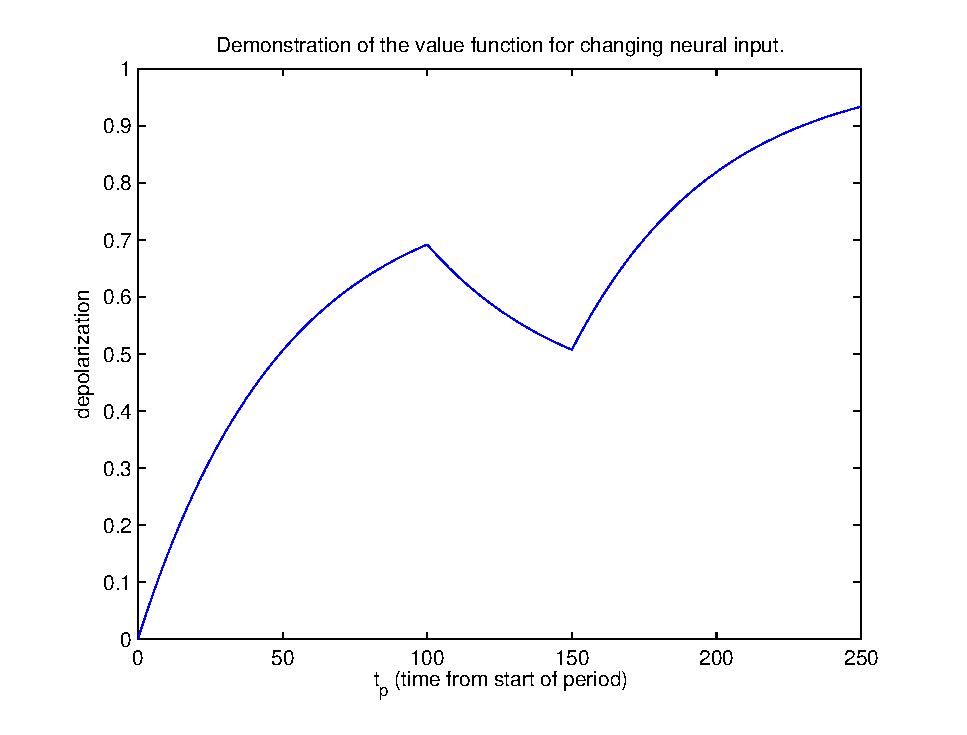
\includegraphics[width=0.95\textwidth]{demonstrasjonAvUlikeKappaforVerdifunksjonen.eps}
	\caption{$v(t)$ for changing $\kappa$. $\kappa_0=0.7$. At time $t_p=100$ $\kappa$ changes to $\kappa_1=0.5$. At time $t_p=150$ the neurons imput increases, and $\kappa$ becomes $\kappa_2=1$. See eq.\eqref{eqVerdiligninga}.}
	\label{figVerdifunksjonen}
\end{figure}

When $\kappa$ is changed, the initial value of the next time window, $v_0$, can be calculated from \eqref{eqVerdiligninga}. 
We can now use \eqref{eqTidTilFyringVedEndraKappa} to find the new estimate for the firing time of the node.
I use the word estimate because we can not know when $\kappa$ will change.
If $\kappa$ is changed before the estimated firing time, the firing time will be affected. 
%XXX if this is before the estimated firing time, the estimate of the next task time will change accordingly.  %If $\kappa$ is changed, the estimate changes.
%-> da er det "but an estimate of firing time.."

%Equation \eqref{eqTidTilFyringVedEndraKappa} gives us the time of firing for a situation where the initial value of the node can be different from zero.
%Also this equation is based on a constant $\kappa$.





%The equations can also be used as the non--linear activation function for a fANN. This activation function is based on a mechanistic model of the biological neuron.
%The activity can be read out of eq. \eqref{eqPeriodeligningForKonstIntraPeriodKAPPA} as the frequency $f(t) = \frac{1}{p(\kappa)}$
%
%If we let the activity level vary between spikes, the model will give as accurate timing as ``Spiking Artificial Neural Network''(SANN). We will discuss different aspects of artificial neural networks later. %XXX Ref?
%The model is based on fundamentally different equations than the model for SANN. 
%If this new model is as effective or more effective than SANN this project will be a contribution because we calculated the firing time in a new way.
%%Ta vekk siste, forrige linje?

%An other aspect with this new model is that it lies between the two prior models of ANN, and can easily communicate with both.

% If we allow the input and activity of each neuron to vary between spikes, the model approaches the model for the biological neuron.
% When $\kappa$ is updated, a new time window starts. 
% $v_0$ from \eqref{eqVerdiligninga} now represents the value at the start of the time window ( $v_0 = v(t=0)$ ). 
% This value is equal to the value $v(t)$ at the time of change of $\kappa$ from the previous time window(se fig. \ref{figVerdifunksjonen}).
% This is equal to the value of the neuron at the time of variation of $\kappa$ (the value at the end of the previous time window).

In fig. \ref{figVerdifunksjonen}, $v(t)$ is simulated for three different time windows. At time $t_p=100$, $\kappa$ changes from $\kappa_0=0.7$ to $\kappa_1=0.5$. At time $t_p=150$, $\kappa$ becomes $\kappa_2=1$. 
The simulation implies that the value function is a continous function that converges toward the neurons final value, $\kappa$, also when $\kappa$ varies.


With this new use of eq. \eqref{eqVerdiligninga}, we can calculate the remaining part of the neurons period after $\kappa$ changes value. 
The remaining time of the period is given by equation \eqref{eqTidTilFyringVedEndraKappa}, given constant $\kappa$. 
If this is updated each time $\kappa$ varies, we get an estimate of the remaining time based on the present $\kappa$.

%Skrive at dette plottet IKKJE er fra kjøring av programmet?




%TODO Finn eit bedre navn på denne subsubsection.
\subsection{The constants in the depolarization equation}
%\subsection{Redying the equation for use in ANN}
%TODO Skriv at denne ligninga kan brukes direkte for å lage en heilt ny modell for "spiking ANN" (ANN med information om 'spike-time').
% 	Om dette skal gjøres, må modellen tilpasses. Blabla, dette gjøres her. Eller noke.. Kanskje ikkje.
\label{sssecValueOfAlpha}

%XXX Veit ikkje om dette er relevant!

The inter--spike interval for a neuron consists of two phases. 
The absolute refraction period and the depolarizing phase (se sec. \ref{ssecTheActionPotential}).

Equation \eqref{eqPeriodeligningForKonstIntraPeriodKAPPA} describes the depolarizing phase of the neuron. % , $p_d(\kappa)$.
The equation for the whole inter--spike interval is given by
\begin{equation}
	p_{isi}(\kappa) = p_d(\kappa) + t_r
\end{equation}

Where $t_r$ is the absolute refraction period of the neuron. % , and $p_d(\kappa)$ is given in \eqref{eqPeriodeligningForKonstIntraPeriodKAPPA}.
If we consider the firing frequency of the neuron, $f(\kappa) = p_{isi}^{-1}(\kappa)$ we can se that the asymptote is given by
\begin{equation}
	\begin{split}
		\lim_{\kappa->\infty}{ f(\kappa)} &= \lim_{\kappa->\inf}\left( \frac{-\alpha}{\ln \left( \frac{\kappa - \tau}{\kappa} \right) - \alpha t_r} \right)   \qquad = \frac{1}{t_r} \\ 
		%\lim_{\kappa->\infty}{ f(\kappa)} &= \frac{1}{t_r}
	\end{split}
\end{equation}

%Using l'Hôpital's rule %INNI ln(-) funksjonen. TODO Viktig å få med dette i denne setninga!
%and get %sjå wolframalpha.com ...
%\begin{equation}
%	\label{eqFrekvensLlim}
%	\lim_{\kappa->\infty}{ f(\kappa}) = \frac{1}{t_r}
%\end{equation}



We can see from this analysis that the refraction period of the neuron is fundamental for restricting the neurons output frequency (se fig. \ref{figFrekvensMedOgUtenRefractionPeriod}).
For biological neurons, the maximum firing frequency is about 1000 Hz \cite{NeuroscienceExploringTheBrain3edKAP4}. %s 79
\begin{equation}
	\lim_{\kappa->\infty}{ f(\kappa}) \approx 1000 \, \text{Hz}
\end{equation}
%If we define the maximum firing frequency to be 1000, equation \ref{eqFrekvensLlim} gives us the absolute refraction period as
We define the maximum firing frequency for the artificial neuron to be 1000 Hz. From equation \ref{eqFrekvensLlim} we get the absolute refraction period as
\begin{equation}
	t_r = \frac{1}{1000 \text{Hz}} = 1 \, \text{m}s %= 0.001 s = 
\end{equation}

%TODO Skriv at dette er en kjendt størrelse i neuroscience (finn, referer), og er en indikasjon på rettheten til lingningene (?)
% 		Kanskje også skrive litt om at dette er "absolute refraction period". Det er også en mild refraction period etter dette (finn,referer). Dette kan implementeres ved 2ms refraction period for auronet. 
% 		TODO TODO Sjekk andre linja her, og gjør en bestemmelse i forhold til mine ANN. (1 eller 2 ms refraction period?).
If we define the time step of the simulation to be 1 m$s$, the refraction period will be one time step in the simulation.
With a time step of 1 m$s$, the absolute refraction period (the time interval where it is impossible to exite the neuron) can be set to one time step. 
For SANN nodes, this means that the node will not change its value for the duration of the next time step. 
For $\kappa$ANN this can be implemented more effective by incrementing the estimated firing time by one time iteration. 
%TODO fullfør!


% Plott av frekvens med, og uten refraction period:
\begin{figure}[bhtp]
	\label{figFrekvensMedOgUtenRefractionPeriod}
	\begin{center}
		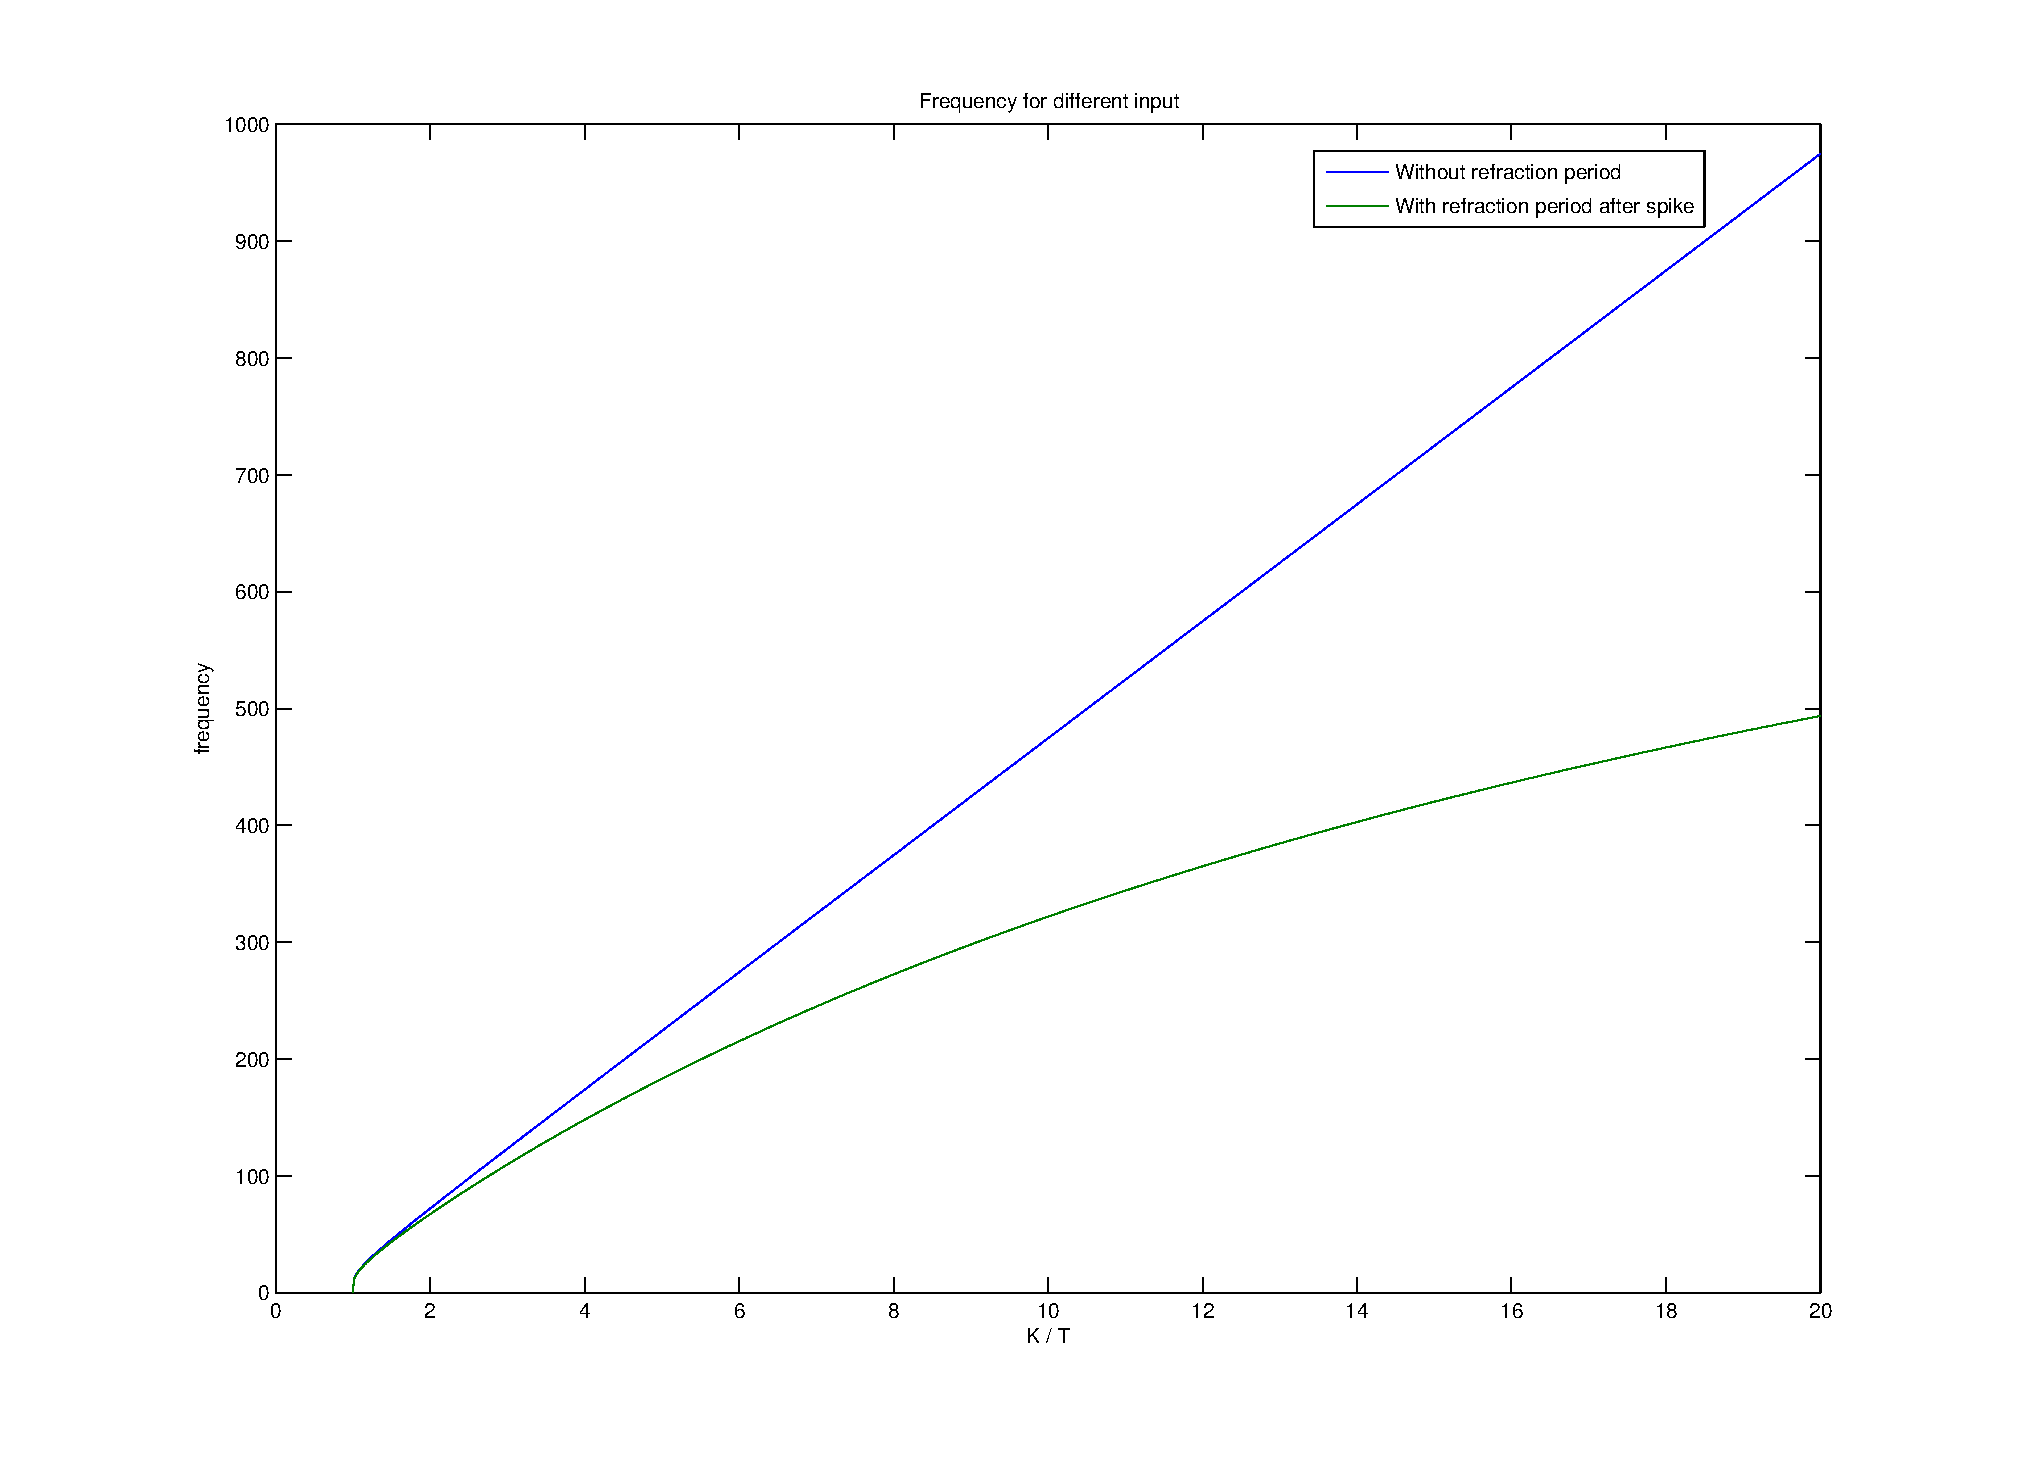
\includegraphics[width=0.95\textwidth]{frekvensPlotRefractionPeriod.eps}
	\end{center}
	\caption{Frequency for a neuron for different values of input. With and without refraction period}
\end{figure}



%TODO Skriv meir om kva de ulike variablane betyr. Kva er \kappa! kva er \tau,\alpha. Skriv om v_0 for tidsvinduet (referer mykje til rett section)



%TODO Skriv om høgare syn på systemet. Kva betyr Kappa (=ett slags mål på input/lekkasje), output gjennom utsynapser er en funksjon som avhenger av [syn.weight]/[isi_intervall].
% 		- får dermed en { alpha*w_{ij} / ln(1-(T/K)) } relasjon mellom neuronets aktivering (K) og neste neurons input. Bør kanskje lese deg opp på "log-summering som multiplikasjon"-artikkelen, og referere!






%********************************************************************************************************************
%********************************************************************************************************************
%*********************     Trur firing cycle skal vekk!  Evt. finn ut korleis det basser inn.  **********************
%********************************************************************************************************************
%********************************************************************************************************************

%mulighet: Kan skrive om det som en måte å visualisere en ide. Sjå for seg en firing cycle, kvar gang $\kappa$ blir oppdatert, regnes \theta ut. Dette gir oss muligheten for å holder oversikt over fase for signalet.
% skriv om firing cycle som eit konsept, tankebane.






%For this we need to introduce a new concept called the firing cycle.

%\subsubsection{The firing cycle}
%(Skriv om firing cycle, men at det er bedre å regne det ut fra verdien fra eq. \eqref{eqVerdiligninga})

%Because of the cyclic nature of the neurons depolarization, it is possible to visualize the neurons interspike period as a firing cycle.
%If we view this as a cycle, the angle $\theta$ can represent the normalized depolarization of the neuron.

%By defining $\omega(\kappa) = \dot{\theta}(\kappa)$ as a function of $\kappa$ over an infinitesimal period of time, the presumption of constant input over the period becomes more realistic. 
%$\kappa$ will then be used to find the derivative of the depolarization of the neuron. For discrete--time systems this infinitesimal period means the least possible time step, one time iteration.

%If we define 
%\begin{equation}
%	\omega(\kappa) = \frac{1}{p(\kappa)}
%\end{equation}

%Since $\omega = \dot{\theta}$, for constant $\kappa$ over some time interval we have that: 
%\begin{equation}
%	\begin{split}
%		\theta^* = \int_0^{t^*} \! \omega(\kappa) \, \mathrm{d}t 		&= 		\int_0^{t^*} \! \frac{1}{ p(\kappa) } \, \mathrm{d}t 	\\
%					\left[\omega(\kappa)\right]_0^{t^*} 				&= 		\left[ \frac{1}{p(\kappa)}\right]_0^{t^*} 				\\
%																	&= 		\frac{t^*}{p(\kappa)}
%	\end{split}
%\end{equation}
%
%We se from this equation that as $t^* = [0,p(\kappa)]$, we have that $\theta=[0,1]$.
%
%Thus $\theta$ represents the normalized depolarization of the neuron. If we for some reason needs to find the depolarization of the neuron this can be calculated by
%\begin{equation}
%	v(t^*) = p(\kappa) \theta^*
%\end{equation}



%If we further introduce the possibility to change $\omega$ an any time during the period, we can sum the contribution of each period with constant $\kappa$:
%%XXX kan vi anta at \theta_0 + \int_0^t \theta dt = \int_{t_0}^t \theta dt ? : JA siden kappa er konstant så varierer ikkje det inne i integralet med integranten (dt)
% 																																									eller ?
%\begin{equation}
%	\begin{split}
%		\theta_{new} = \theta_{old} + \int_{t_0}^{t^*} \! \omega \, \mathrm{d}t 	\qquad \text{stemmer dette?} %	&= 		\int_0^{t^*} \! \frac{1}{ p(\kappa) } \, \mathrm{d}t 	
%	\end{split}
%\end{equation}

%For a discrete--time system the smallest timestep is defined as one time iteration. For such systems we get:
%\begin{equation}
%	\begin{split}
%		\theta^* = \sum_0^{t_n^*} \! \omega  		&= 		\sum_0^{t_n^*} \! \frac{1}{ p(\kappa) } 	\\
%					\left[\omega\right]_0^{t_n^*} 	&= 		\left[ \frac{1}{p(\kappa)}\right]_0^{t_n^*}	\\
%													&= 		\frac{t_n^*}{p(\kappa)}
%	\end{split}
%\end{equation}

%NESTE: Skriv korleis vi kan la input variere når vi gjekk ut fra at input var konstant. 	-- 'Firin cycle'











%XXX XXX XXX kva er forskjellen mellom denne modellen og SANN? Denne modellen holder input fra kvart inputneuron konstant mellom dets spiker(?) mens SANN holder lekkasjen konstant over kvar tidsiterasjon.





